\chapter{Cadre général}
\label{sec:Cadre général}

\section{Présentation de l’Entreprise}

\subsection{Le LRI}
Le Laboratoire de Recherche en Informatique(LRI) est une unité de recherche de l'Université Paris Sud en partenariat avec le CNRS, le Centre National de la Recherche Scientifique, l'INRIA et Centrale / Supelec. Fondé il y a plus de 35 ans, il compte plus de 250 membres, dont plus de 130 professeurs et membres du personnel et 88 doctorants. Le LRI se compose de neuf groupes de recherche, soutenus par un personnel administratif et technique. Quatre des groupes de recherche sont totalement ou partiellement associés à Inria Saclay Ile de France, ce qui en fait l'un des principaux partenaires du laboratoire. Le laboratoire est situé sur le plateau de Moulon dans ses nouveaux bâtiments connectés Ada Lovelace et Claude Shannon.

Les thèmes de recherche du laboratoire couvrent un large spectre de l'informatique à dominante logicielle et incluent à la fois des aspects fondamentaux et des aspects appliqués : algorithmique, combinatoire, graphes, optimisation discrète et continue, programmation, génie logiciel, vérification et preuves,  parallélisme, calcul à haute performance, grilles, architecture et compilation, réseaux, bases de données, représentation et traitement des connaissances, apprentissage, fouille de données, bioinformatique, interaction homme-machine, etc.  Cette diversité est l'une des forces du laboratoire car elle favorise les recherches aux frontières, là où le potentiel d'innovation est le plus grand.

Le laboratoire participe à un grand nombre de projets nationaux et internationaux, notamment ceux financés par l'Agence National de la Recherche (ANR), par Digiteo et par l'Union européenne (notamment la CCI ICT Labs de l'EIT). Les membres du LRI participent à de nombreux comités éditoriaux de revues internationales et comités de programme de conférences internationales. Le laboratoire a également une très forte activité de publication avec plus de 2000 publications entre début 2008 et mi 2013 ainsi qu'une importante activité de production logicielle et de transfert.

Le LRI fait partie de Digiteo l'un des douze réseaux de recherche créés par le gouvernement français en 2007 et le seul en sciences et technologies de l'information (STIC). Digiteo rassemble sur le plateau de Saclay 1200 chercheurs issus de 23 laboratoires de six instituts nationaux de recherche fondateurs (CNRS, CEA, Inria, Université Paris-Sud, Ecole Polytechnique, Supélec) et de six membres associés (Ecole Centrale Paris, ENS Cachan, Université de Versailles Saint Quentin en Yvelines, Institut Mines-Télécom, Mines ParisTech, ENSTA ParisTech). Le LRI est également partenaire de System@tic Paris-Région, un pôle de compétitivité de classe mondiale regroupant plus de 200 industriels, universitaires et institutionnels dans le domaine des logiciels et systèmes complexes.

Le LRI est fortement impliqué dans les programmes d'Investissements d'Avenir lancés en 2010 par le gouvernement français. Il dirige l'Equipex Digiscope, du Labex Digicosme qui participe à l'IRT SystemX et est très actif dans l'Idex Paris-Saclay qui donnera naissance en 2014 à la nouvelle Université Paris-Saclay: Le LRI joue un rôle important dans la mise en place du futur département STIC dans la continuité de Digiteo et dirige les projets de l'Ecole Doctorale STIC et du Master Informatique de l'Université Paris-Saclay.

\subsection{Chiffres clés}

Le LRI compte plus de 250 membres, dont plus de 112 professeurs permanents, 88 doctorants, 27 ingénieurs, techniciens, personnel administratif. Ses menbres ont durant la période 2010-2014 effectué plus de 2000 publications. Le LRI est un partenaire académique d'envergure international avec des partenarias avec des universités préstigieuse dont notamment l'Université de Tokyo, l'Université de Montréal,  l'Université d'Oxford, l'Université de Californie à Berkeley, l'Université de Vienne Autriche,... L'une des forces du laboratoire est d'avoir des partenaires industriels de choix tels que :  EDF,Thalès,Nokia, Philips, L'oréal, IBM, Schneider, SAP Sirehna qui permettent aux chercheurs d'être connectés avec la réalité industrielle et ses enjeux. 


\subsection{Organisation et l'equipe MODHEL}

Le Laboratoire de Recherche informatique est composé de 9 équipes de recherche. J'ai effectué mon stage au sein de l'équipe Modélisation Hétérogène (MODHEL) dirigé par Frédéric BOULANGER. Chaque équipe de recherche travaille soit sur un logiciel et brevet soit sur une thèses ou une habilitations récentes.

\begin{figure}[htp]
  \centering
  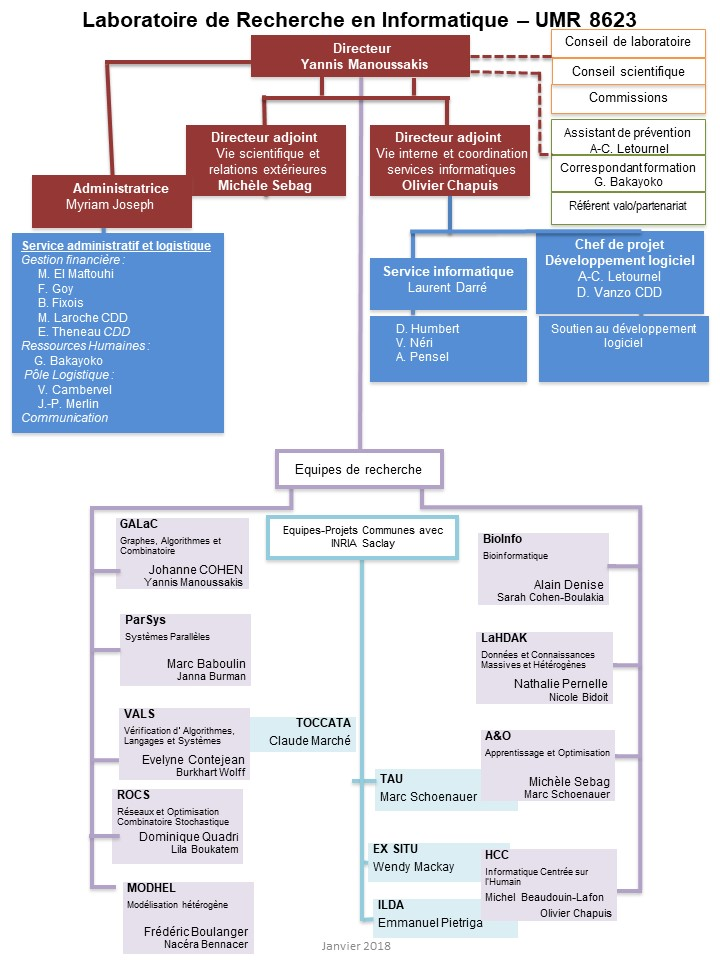
\includegraphics[width=7cm]{images/Orga_LRI}
  \caption{Organigramme du LRI.}
  \label{fig:une-autre-image}
\end{figure}

Mon sujet de stage m’a conduit à travailler sur la thèse de Julien HAY qui s'intitule : "Analyse des réseaux sociaux pour enrichir et segmenter les profils utilisateurs. Cette thèse en préparation à Paris Saclay , dans le cadre de Sciences et Technologies de l'Information et de la Communication , en partenariat avec le LRI au sein de l'équipe de recherche MODHEL et Central Supélec  (établissement de préparation de la thèse) depuis le 20-03-2017. Durant mon stage, mon équipe de travail au sein de l’équipe MODHEL est composé de Julien HAY qui est donc un doctorant mais aussi  mon tuteur de stage et Alexis JODAR un étudiant en 3ième année d’étude au sein de l’école epitech qui va s’occuper du back-end de l’application 


\subsection{Résumé de la thèse de J. HAY}

Le travail de recherche de Julien HAY vise à améliorer et à développer de nouveaux algorithmes de segmentation et d'enrichissement des profils utilisateurs tout en validant leur application dans le cadre de la plateforme industrielle Octopeek. Octopeek est une startup spécialisée en Big Data et Data Science. Dans le cadre de cette thèse, il est prévu de mettre en place des méthodes d'extraction et d'analyse des données internes aux réseaux sociaux mais également issues d'autres sources de données en vue de leur réutilisation dans la plateforme Octopeek. Néanmoins, la réalisation d'un tel système demeure un défi scientifique qui devra prendre en compte le volume de données, le temps d'exécution de la recherche et la sémantique des termes afin de fournir les meilleures réponses. En effet, pour chaque information recherchée, il faudra trouver la méthode, l'algorithme optimisé qui prend en compte la rapidité de calcul, et le scoring associé. A terme il sera amené à implémenter des algorithmes pour une utilisation à la volée et sur plusieurs personnes en parallèle.


\section{Sujet du stage}

\subsection{Missions et enjeux}

L'objectif premier de ce stage est le développement d’une application mobile qui présentera des articles d’actualité aux utilisateurs selon leurs intérêts. L’application devra être multi-plateforme : Android et iOS et devra permettre l’évaluation de différents systèmes de recommandation grâce à des métriques telles que CTR (Click-through rate). Avec l’accord de chaque utilisateur, une analyse précise de leur navigation (géolocalisation, temps de lecture, scroll des articles. . .) et comportement permettra de capturer des éléments de contexte et des retours de pertinence implicites utiles aux algorithmes de recommandation. Chaque utilisateur sera identifié par son profil sur les réseaux sociaux (Facebook, Twitter) ou via une adresse mail. Dans une seconde partie du stage, il est prévu de construire un système de recommandation baseline s’appuyant sur les activités passées de chaque utilisateur, ainsi que sur une base de données d’articles renouvelée en temps réel. Ce travail sera réalisé sous la supervision du doctorant en charge du projet et en collaboration avec un second stagiaire réalisant la partie architecture et récolte de données (notamment pour alimenter la base de données d’articles). 

\subsection{Problématique}

Les recherches dans le domaine des systèmes de recommandation s’appuient la plupart du temps sur des évaluations “offline” qui ne permettent pas d’établir des métriques en phase avec une réelle satisfaction utilisateur. Dans le sous-domaine de la recommandation d’articles d’actualité, il existe à ce jour très peu de systèmes permettant aux différentes équipes de recherche de tester leurs algorithmes en temps réel, i.e. sur des utilisateurs interagissant directement avec le système de recommandation. 


Nous proposons de développer une application mobile qui tentera de contourner ces obstacles et  permettra dans un premier temps, l’évaluation de nos algorithmes de recommandation sur des utilisateurs en contexte et en temps réel. Et permettra, dans un second temps la confrontation de différentes équipes de recherche du domaine.




%%% Local Variables: 
%%% mode: latex
%%% TeX-master: "lri-report"
%%% End: 